%%%%%%%%%%%%%%%%%%%%%%%%%%%%%%%%%%%%%%%%%
% Beamer Presentation
% LaTeX Template
% Version 1.0 (10/11/12)
%
% This template has been downloaded from:
% http://www.LaTeXTemplates.com
%
% License:
% CC BY-NC-SA 3.0 (http://creativecommons.org/licenses/by-nc-sa/3.0/)
%
%%%%%%%%%%%%%%%%%%%%%%%%%%%%%%%%%%%%%%%%%

%----------------------------------------------------------------------------------------
%	PACKAGES AND THEMES
%----------------------------------------------------------------------------------------

\documentclass[handout]{beamer}

\mode<presentation> {

% The Beamer class comes with a number of default slide themes
% which change the colors and layouts of slides. Below this is a list
% of all the themes, uncomment each in turn to see what they look like.

%\usetheme{default}
%\usetheme{AnnArbor}
%\usetheme{Antibes}
%\usetheme{Bergen}
%\usetheme{Berkeley}
%\usetheme{Berlin}
%\usetheme{Boadilla}
%\usetheme{CambridgeUS}
%\usetheme{Copenhagen}
%\usetheme{Darmstadt}
%\usetheme{Dresden}
%\usetheme{Frankfurt}
%\usetheme{Goettingen}
%\usetheme{Hannover}
%\usetheme{Ilmenau}
%\usetheme{JuanLesPins}
%\usetheme{Luebeck}
\usetheme{Madrid}
%\usetheme{Malmoe}
%\usetheme{Marburg}
%\usetheme{Montpellier}
%\usetheme{PaloAlto}
%\usetheme{Pittsburgh}
%\usetheme{Rochester}
%\usetheme{Singapore}
%\usetheme{Szeged}
%\usetheme{Warsaw}

% As well as themes, the Beamer class has a number of color themes
% for any slide theme. Uncomment each of these in turn to see how it
% changes the colors of your current slide theme.

%\usecolortheme{albatross}
%\usecolortheme{beaver}
%\usecolortheme{beetle}
%\usecolortheme{crane}
%\usecolortheme{dolphin}
%\usecolortheme{dove}
%\usecolortheme{fly}
%\usecolortheme{lily}
%\usecolortheme{orchid}
%\usecolortheme{rose}
%\usecolortheme{seagull}
%\usecolortheme{seahorse}
%\usecolortheme{whale}
%\usecolortheme{wolverine}

%\setbeamertemplate{footline} % To remove the footer line in all slides uncomment this line
%\setbeamertemplate{footline}[page number] % To replace the footer line in all slides with a simple slide count uncomment this line

%\setbeamertemplate{navigation symbols}{} % To remove the navigation symbols from the bottom of all slides uncomment this line
}

\usepackage{graphicx} % Allows including images
\usepackage{booktabs} % Allows the use of \toprule, \midrule and \bottomrule in tables
\usepackage{cool}
\usepackage{tikz}
\usepackage{amsmath}
\usepackage{listings}
\DeclareMathOperator*{\argmax}{argmax}
\DeclareMathOperator*{\argmin}{argmin}
\usetikzlibrary{positioning}

%----------------------------------------------------------------------------------------
%	TITLE PAGE
%----------------------------------------------------------------------------------------


\title[Asset-Allocation Chapter]{A Guided Tour of \href{http://stanford.edu/~ashlearn/RLForFinanceBook/book.pdf}{\underline{\textcolor{yellow}{Chapter 6}}}: \\  Dynamic Asset-Allocation and Consumption} 

\author{Ashwin Rao} % Your name
\institute[Stanford] % Your institution as it will appear on the bottom of every slide, may be shorthand to save space
{
ICME, Stanford University
 % Your institution for the title page
}

\date{\today} % Date, can be changed to a custom date

\begin{document}
\begin{frame}
\titlepage % Print the title page as the first slide
\end{frame}

\begin{frame}
\frametitle{Dynamic Asset-Allocation and Consumption}
\pause
\begin{itemize}[<+->]
\item The broad topic is Investment Management
\item Applies to Corporations as well as Individuals
\item The two considerations are:
\pause
\begin{itemize}[<+->]
\item How to allocate money across assets in one's investment portfolio
\item How much to consume for one's needs/operations/pleasures
\end{itemize}
\item We consider the dynamic version of these dual considerations
\item Asset-Allocation and Consumption decisions at each time step
\item Asset-Allocation decisions typically deal with Risk-Reward tradeoffs
\item Consumption decisions are about spending now or later
\item Objective: Horizon-Aggregated Expected Utility of Consumption
\end{itemize}
\end{frame}

\begin{frame}
\frametitle{Let's consider the simple example of Personal Finance}
\pause
\begin{itemize}[<+->]
\item Broadly speaking, Personal Finance involves the following aspects:
\pause
\begin{itemize}[<+->]
\item Receiving Money: Salary, Bonus, Rental income, Asset Liquidation etc.
\item Consuming Money: Food, Clothes, Rent/Mortgage, Car, Vacations etc.
\item Investing Money: Savings account, Stocks, Real-estate, Gold etc.
\end{itemize}
\item Goal: Maximize lifetime-aggregated Expected Utility of Consumption
\item This can be modeled as a Markov Decision Process
\item {\em State:} Age, Asset Holdings, Asset Valuation, Career situation etc.
\item {\em Action:} Changes in Asset Holdings, Optional Consumption
\item {\em Reward:} Utility of Consumption of Money
\item {\em Model:} Career uncertainties, Asset market uncertainties
\end{itemize}
\end{frame}

\begin{frame}
\frametitle{Merton's Frictionless Continuous-Time Formulation}
\pause
\begin{itemize}[<+->]
\item Assume: Current wealth is $W_0 > 0$, and you'll live for $T$ more years
\item You can invest in (allocate to) $n$ risky assets and a riskless asset
\item Each risky asset has known normal distribution of returns
\item Allowed to long or short any fractional quantities of assets
\item Trading in continuous time $0 \leq t < T$, with no transaction costs
\item You can consume any fractional amount of wealth at any time
\item Dynamic Decision: Optimal Allocation and Consumption at each time
\item To maximize lifetime-aggregated Expected Utility of Consumption
\item Consumption Utility assumed to have Constant Relative Risk-Aversion
\end{itemize}
\end{frame}

\begin{frame}
\frametitle{Problem Notation}
For simplicity, we state and solve the problem for 1 risky asset but the solution generalizes easily to $n$ risky assets.
\pause
\begin{itemize}[<+->]
\item Riskless asset: $dR_t = r \cdot R_t \cdot dt$
\item Risky asset: $dS_t = \mu \cdot S_t \cdot dt + \sigma \cdot S_t \cdot dz_t$ (i.e. Geometric Brownian)
\item $\mu > r > 0, \sigma > 0$ (for $n$ assets, we work with a covariance matrix)
\item Wealth at time $t$ is denoted by $W_t > 0$
\item Fraction of wealth allocated to risky asset denoted by $\pi(t, W_t)$
\item Fraction of wealth in riskless asset will then be $1 - \pi(t, W_t)$
\item Wealth consumption per unit time denoted by $c(t, W_t) \geq 0$
\item Utility of Consumption function $U(x) = \frac {x^{1-\gamma}} {1 - \gamma}$ for $0 < \gamma \neq 1$
\item Utility of Consumption function $U(x) = \log(x)$ for $\gamma = 1$
\item $\gamma =$ (Constant) Relative Risk-Aversion $\frac {-x \cdot U''(x)} {U'(x)}$
\end{itemize}
\end{frame}

\begin{frame}
\frametitle{Formal Problem Statement}
\pause
\begin{itemize}[<+->]
\item We write $\pi_t, c_t$ instead of $\pi(t, W_t), c(t, W_t)$ to lighten notation
\item Balance constraint implies the following process for Wealth $W_t$
$$dW_t = ((\pi_t \cdot (\mu - r) + r) \cdot W_t - c_t) \cdot dt + \pi_t \cdot \sigma \cdot W_t \cdot dz_t$$
\item At any time $t$, determine optimal $[\pi(t,W_t), c(t, W_t)]$ to maximize:
$$\mathbb{E}[\int_t^T \frac {e^{-\rho (s-t)} \cdot c_s^{1-\gamma}} {1-\gamma} \cdot ds + \frac {e^{-\rho (T-t)} \cdot B(T) \cdot W_T^{1-\gamma}} {1-\gamma} \mid W_t]$$
\item where $\rho \geq 0$ is the utility discount rate, $B(T)$ is the bequest function
\item We can solve this problem for arbitrary bequest $B(T)$ but for simplicity, will consider $B(T) = \epsilon^{\gamma}$
where $0 < \epsilon \ll 1$, meaning ``no bequest'' (we need this $\epsilon$-formulation for technical reasons).
\item We will solve this problem for $\gamma \neq 1$ ($\gamma = 1$ is easier, hence omitted)
\end{itemize}
\end{frame}

\begin{frame}
\frametitle{Continuous-Time Stochastic Control}
\begin{itemize}[<+->]
\item Think of this as a continuous-time Stochastic Control problem
\item The {\em State} at time $t$ is $(t, W_t)$
\item The {\em Action} at time $t$ is $[\pi_t, c_t]$
\item The {\em Reward} per unit time at time $t$ is $U(c_t) = \frac {c_t^{1 - \gamma}} {1 - \gamma}$ 
\item The {\em Return} at time $t$ is the accumulated discounted {\em Reward}:
$$\int_t^T e^{-\rho(s-t)} \cdot \frac {c_s^{1-\gamma}} {1-\gamma} \cdot ds$$
\item Find {\em Policy} $: (t, W_t) \rightarrow [\pi_t, c_t]$ that maximizes the {\em Expected Return}
\item Note: $c_t \geq 0$, but $\pi_t$ is unconstrained
\end{itemize}
\end{frame}


\begin{frame}
\frametitle{Optimal Value Function}
\begin{itemize}[<+->]
\item Value Function for a {\em State} (under a given policy) is the {\em Expected Return} from the {\em State} (when following the given policy)
\item We focus on the Optimal Value Function $V^*(t, W_t)$
$$V^*(t, W_t) = \max_{\pi, c} \mathbb{E}_t[\int_t^T \frac {e^{-\rho (s-t)} \cdot c_s^{1-\gamma}}{1 - \gamma} \cdot ds + \frac {e^{-\rho (T-t)} \cdot \epsilon^{\gamma} \cdot W_T^{1-\gamma}} {1 - \gamma} ]$$
\item $V^*(t, W_t)$ satisfies a simple recursive formulation for $0 \leq t < t_1 < T$
$$V^*(t, W_t) = \max_{\pi, c} \mathbb{E}_t[ \int_t^{t_1} \frac {e^{-\rho (s-t)} \cdot c_s^{1-\gamma}} {1 - \gamma} \cdot ds + e^{-\rho(t_1-t)} \cdot V^*(t_1, W_{t_1})]$$
\pause
$$\Rightarrow e^{-\rho t} \cdot V^*(t, W_t) = \max_{\pi, c} \mathbb{E}_t[ \int_t^{t_1} \frac {e^{-\rho s} \cdot c_s^{1-\gamma}} {1 - \gamma} \cdot ds + e^{-\rho t_1} \cdot V^*(t_1, W_{t_1})]$$
\end{itemize}
\end{frame}

\begin{frame}
\frametitle{HJB Equation for Optimal Value Function}
\pause
Rewriting in stochastic differential form, we have the HJB formulation
$$\max_{\pi_t, c_t} \mathbb{E}_t[d(e^{-\rho t} \cdot V^*(t, W_t)) + \frac {e^{-\rho t} \cdot c_t^{1-\gamma}}{1 - \gamma} \cdot dt] = 0$$
\pause
$$\Rightarrow \max_{\pi_t, c_t} \mathbb{E}_t[dV^*(t, W_t) + \frac {c_t^{1-\gamma}}{1 - \gamma} \cdot dt] = \rho \cdot V^*(t, W_t) \cdot dt$$
\pause
Use Ito's Lemma on $dV^*$, remove the $dz_t$ term since it's a martingale, and divide throughout by $dt$ to produce the HJB Equation in PDE form:
$$\max_{\pi_t, c_t} [\pderiv{V^*}{t} + \pderiv{V^*}{W} ((\pi_t (\mu - r) + r)W_t  - c_t)+ \pderiv[2]{V^*}{W} \cdot \frac {\pi_t^2 \sigma^2 W_t^2} {2} + \frac {c_t^{1-\gamma}}{1 - \gamma}]$$
$$ = \rho \cdot V^*(t, W_t)$$
\pause
Let us write the above equation more succinctly as:
$$\max_{\pi_t, c_t} \Phi(t, W_t; \pi_t, c_t) = \rho \cdot V^*(t, W_t)$$
\pause
Note: we are working with the constraints $W_t > 0, c_t \geq 0$ for $0 \leq t < T$
\end{frame}

\begin{frame}
\frametitle{Optimal Allocation and Consumption}
Find optimal $\pi_t^*, c_t^*$ by taking partial derivatives of $\Phi(t, W_t; \pi_t, c_t)$ with respect to $\pi_t$ and $c_t$, and equate to 0 (first-order conditions for $\Phi$).
\pause
\begin{itemize}[<+->]
\item Partial derivative of $\Phi$ with respect to $\pi_t$:
$$(\mu -r) \cdot \pderiv{V^*}{W_t} + \pderiv[2]{V^*}{W_t} \cdot \pi_t \cdot \sigma^2 \cdot W_t = 0$$
$$ \Rightarrow \pi_t^* = \frac {-\pderiv{V^*}{W_t} \cdot (\mu - r)} {\pderiv[2]{V^*}{W_t} \cdot \sigma^2 \cdot W_t}$$
\item Partial derivative of $\Phi$ with respect to $c_t$:
$$-\pderiv{V^*}{W_t} +  (c_t^*)^{-\gamma} = 0$$
$$ \Rightarrow c_t^* = (\pderiv{V^*}{W_t})^{\frac {-1} {\gamma}}$$
\end{itemize}
\end{frame}

\begin{frame}
\frametitle{Optimal Value Function PDE}
\pause
Now substitute $\pi_t^*$ and $c_t^*$ in $\Phi(t, W_t; \pi_t, c_t)$ and equate to $\rho V^*(t,W_t)$, which gets us the Optimal Value Function PDE:
\pause
$$\pderiv{V^*}{t} - \frac {(\mu - r)^2}{2 \sigma^2} \cdot \frac {(\pderiv{V^*}{W_t})^2} {\pderiv[2]{V^*}{W_t}}  + \pderiv{V^*}{W_t} \cdot r \cdot W_t + \frac {\gamma} {1 - \gamma} \cdot (\pderiv{V^*}{W_t})^{\frac {\gamma-1} {\gamma}} = \rho V^*$$ 
\pause
The boundary condition is:
$$V^*(T, W_T) = \epsilon^{\gamma} \cdot \frac {W_T^{1-\gamma}} {1- \gamma}$$
\pause
The second-order conditions for $\Phi$ are satisfied {\bf under the assumptions} $c^*_t > 0, W_t > 0, \pderiv[2]{V^*}{W_t} < 0$ for all $0 \leq t < T$ (we will later show that these are all satisfied in the solution we derive), and for concave $U(\cdot)$, i.e., $\gamma > 0$
\end{frame}

\begin{frame}
\frametitle{Solving the PDE with a guess solution}
\pause
We surmise with a guess solution
$$V^*(t, W_t) = f(t)^{\gamma} \cdot \frac {W_t^{1-\gamma}} {1-\gamma}$$
\pause
Then,
$$\pderiv{V^*}{t} = \gamma \cdot f(t)^{\gamma-1} \cdot f'(t) \cdot  \frac {W_t^{1-\gamma}} {1-\gamma}$$
\pause
$$\pderiv{V^*}{W_t} = f(t)^{\gamma} \cdot W_t^{-\gamma}$$
\pause
$$\pderiv[2]{V^*}{W_t} = - f(t)^{\gamma} \cdot \gamma \cdot W_t^{-\gamma-1}$$
\end{frame}

\begin{frame}
\frametitle{PDE reduced to an ODE}
\pause
Substituting the guess solution in the PDE, we get the simple ODE:
$$f'(t) = \nu \cdot f(t) - 1$$
\pause
where $$\nu = \frac {\rho - (1 - \gamma) \cdot (\frac {(\mu - r)^2} {2 \sigma^2 \gamma} + r)} {\gamma}$$
\pause
with boundary condition $f(T) = \epsilon$.
\pause
\linebreak
The solution to this ODE is:
$$
f(t) =
\begin{cases}
\frac {1 + (\nu \epsilon - 1) \cdot e^{-\nu (T-t)}} {\nu} & \text{for } \nu \neq 0 \\
T-t+\epsilon & \text{for } \nu = 0 \\
\end{cases}
$$
\end{frame}

\begin{frame}
\frametitle{Optimal Allocation and Consumption}
\pause
Putting it all together (substituting the solution for $f(t)$), we get:
$$\pi^*(t, W_t) = \frac {\mu - r} {\sigma^2 \gamma}$$
\pause
$$
c^*(t, W_t)= \frac {W_t} {f(t)} = 
\begin{cases}
\frac {\nu \cdot W_t} {1 + (\nu \epsilon - 1) \cdot e^{-\nu (T-t)}} & \text{for } \nu \neq 0\\
\frac {W_t} {T-t+\epsilon} & \text{for } \nu = 0\\
\end{cases}
$$
\pause
$$
V^*(t, W_t) = 
\begin{cases}
\frac {(1 + (\nu \epsilon - 1) \cdot e^{-\nu (T-t)})^{\gamma}} {\nu^{\gamma}} \cdot \frac {W_t^{1-\gamma}} {1-\gamma} & \text{for } \nu \neq 0\\
\frac {(T-t+\epsilon)^\gamma \cdot W_t^{1 - \gamma}} {1-\gamma} & \text{for } \nu = 0\\
\end{cases}
$$
\pause
\begin{itemize}[<+->]
\item $f(t) > 0$ for all $0 \leq t < T$ (for all $\nu$) ensures $W_t, c^*_t > 0, \pderiv[2]{V^*}{W_t} < 0$. This ensures the constraints $W_t > 0$ and $c_t \geq 0$ are satisfied and the second-order conditions for $\Phi$ are also satisfied.
\item The HJB Formulation was key and this solution approach provides a template for similar continuous-time stochastic control problems.
\end{itemize}
\end{frame}



\begin{frame}
\frametitle{Gaining Insights into the Solution}
\pause
\begin{itemize}[<+->]
\item Optimal Allocation $\pi^*(t, W_t)$ is constant (independent of $t$ and $W_t$)
\item Optimal Fractional Consumption $\frac {c^*(t, W_t)} {W_t}$ depends only on $t$ ($=\frac 1 {f(t)}$)
\item With Optimal Allocation \& Consumption, the Wealth process is:
$$\frac {dW_t} {W_t} = (r + \frac {(\mu - r)^2} {\sigma^2 \gamma} - \frac 1 {f(t)}) \cdot dt + \frac {\mu - r} {\sigma \gamma} \cdot dz_t$$
\item Expected Portfolio Return is constant over time ($=r + \frac {(\mu - r)^2} {\sigma^2 \gamma}$)
\item Assuming $\epsilon < \frac 1 {\nu}$, Fractional Consumption $\frac 1 {f(t)}$ increases over time
\item Expected Rate of Wealth Growth $r + \frac {(\mu - r)^2} {\sigma^2 \gamma} - \frac 1 {f(t)}$ decreases over time
\item If $r + \frac {(\mu - r)^2} {\sigma^2 \gamma} > \frac 1 {f(0)}$, we start by Consuming $<$ Expected Portfolio Growth and over time, we Consume $>$ Expected Portfolio Growth
\item Wealth Growth Volatility is constant ($= \frac {\mu - r} {\sigma \gamma}$)
\end{itemize}
\end{frame}

\begin{frame}
\frametitle{Fractional Consumption and Expected Wealth Growth}
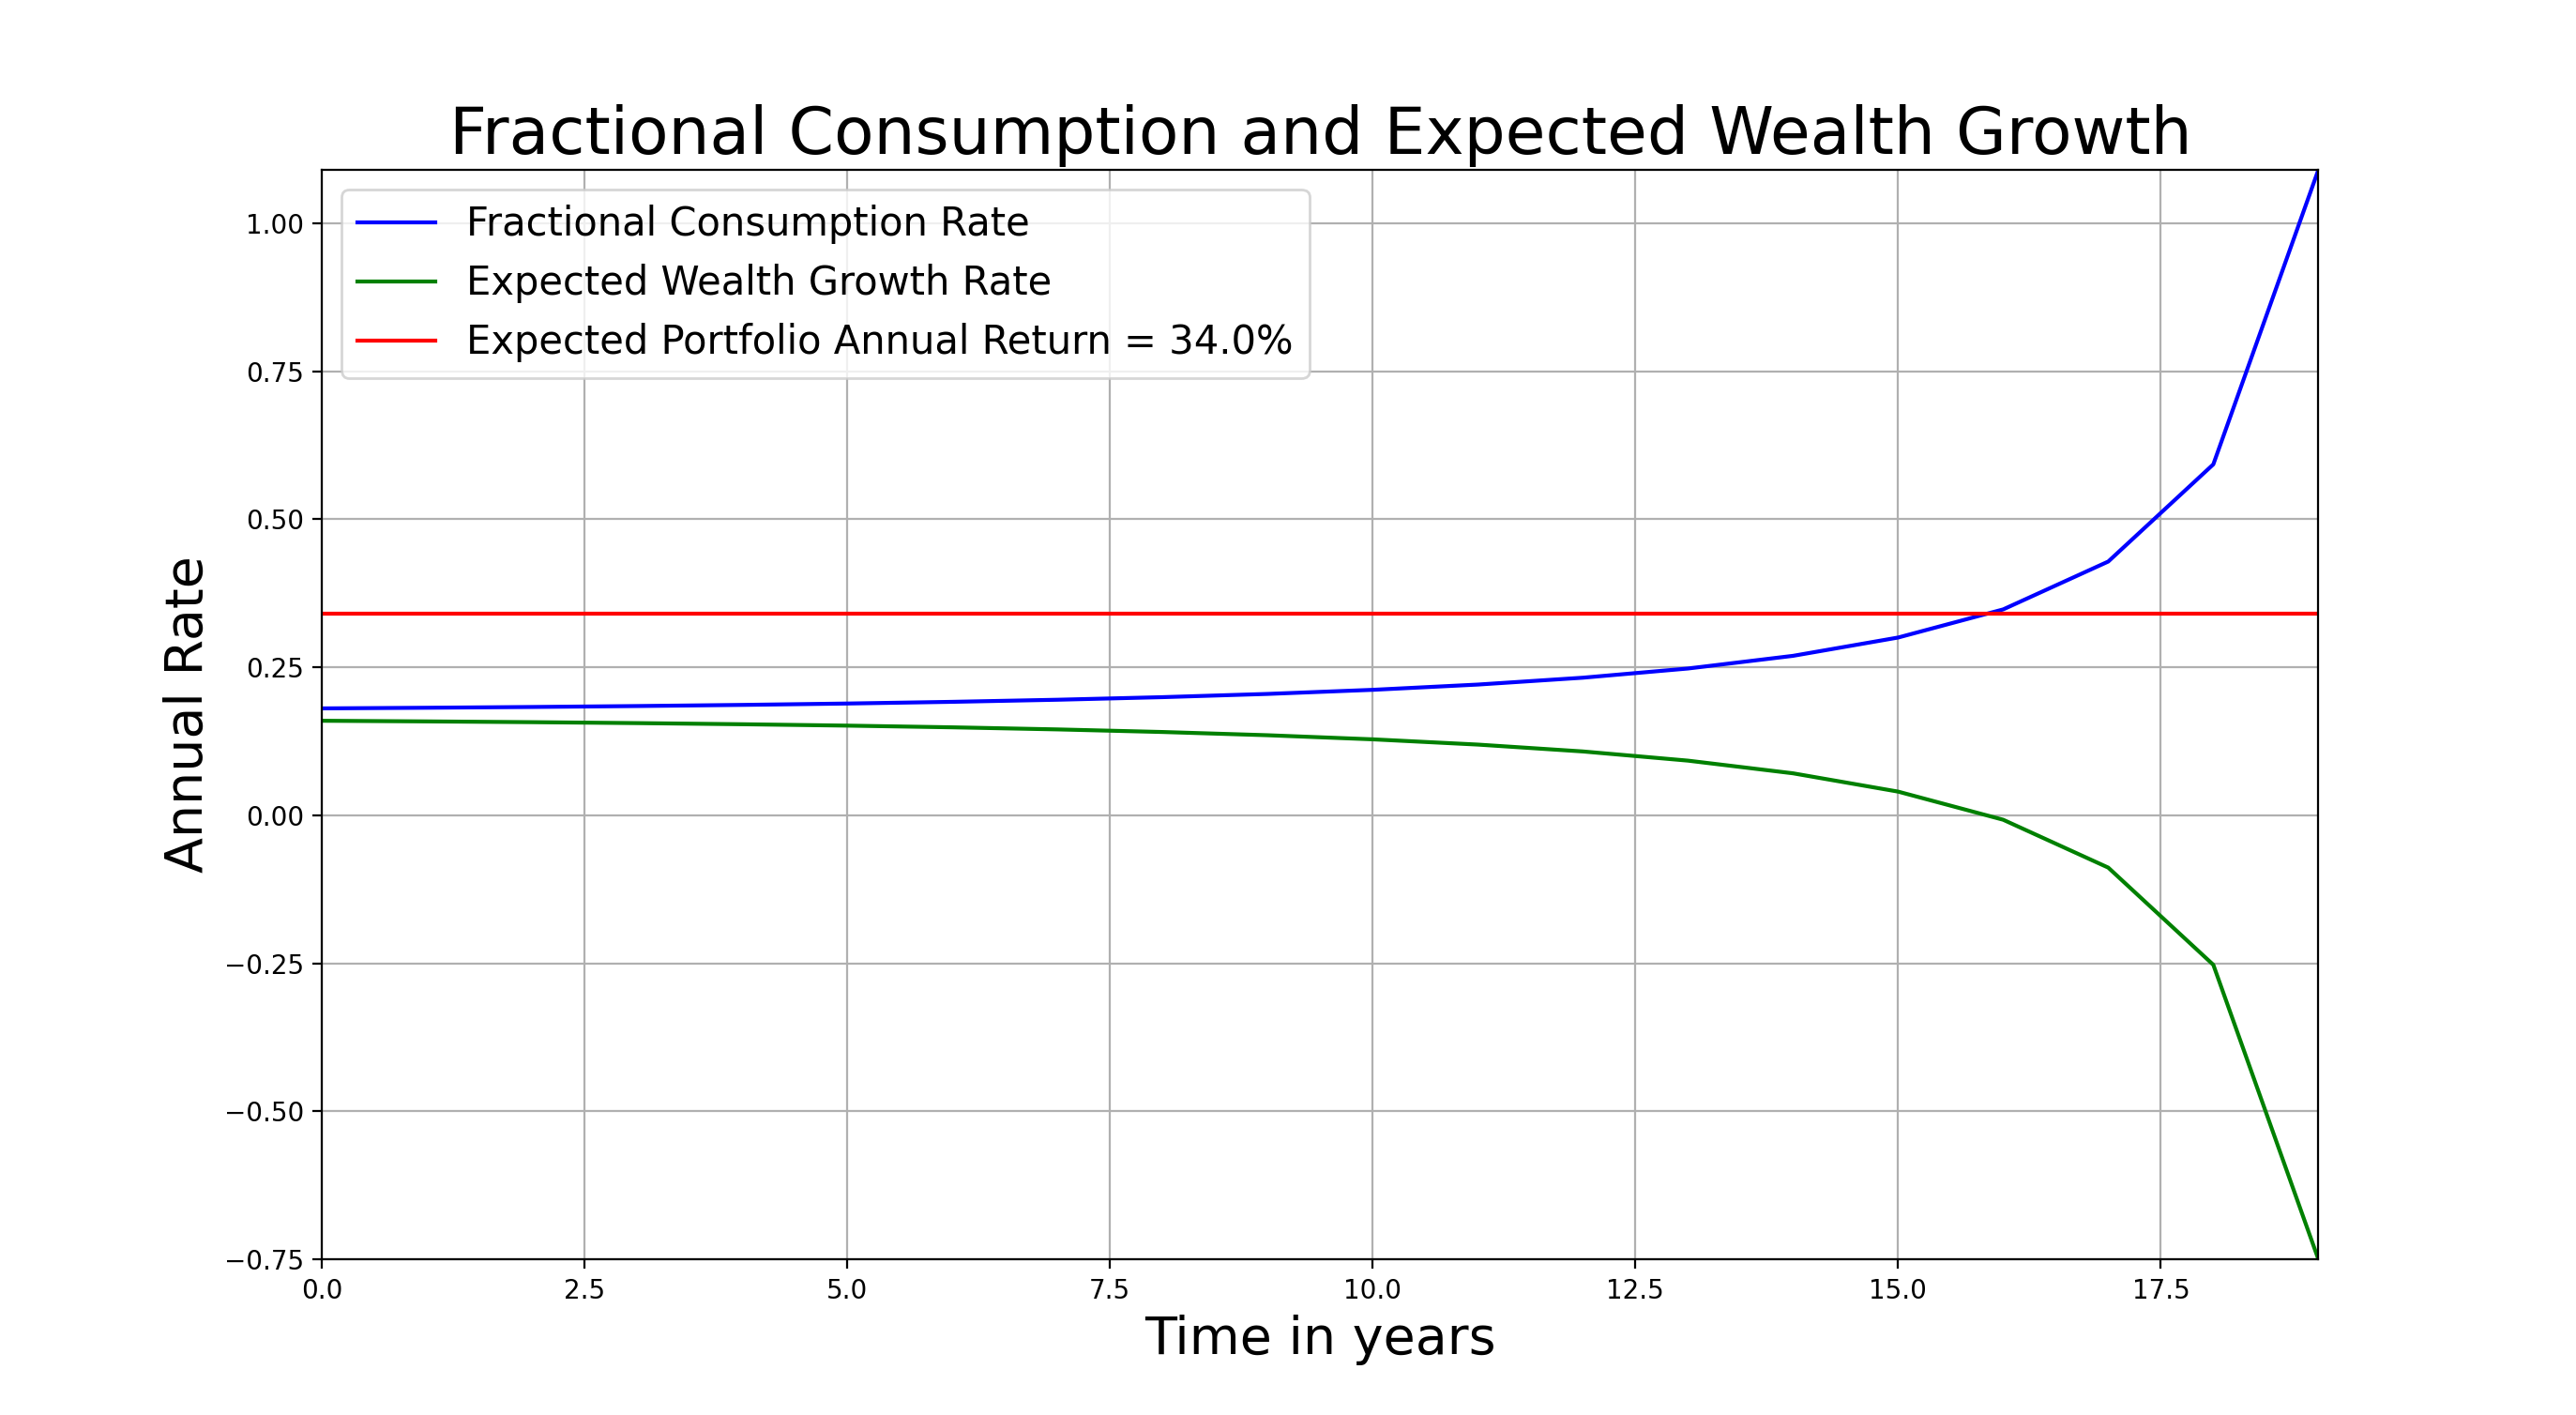
\includegraphics[width=12cm, height=8cm]{portfolio_growth.png}
\end{frame}

\begin{frame}
\frametitle{Time-Trajectory of Expected Wealth}
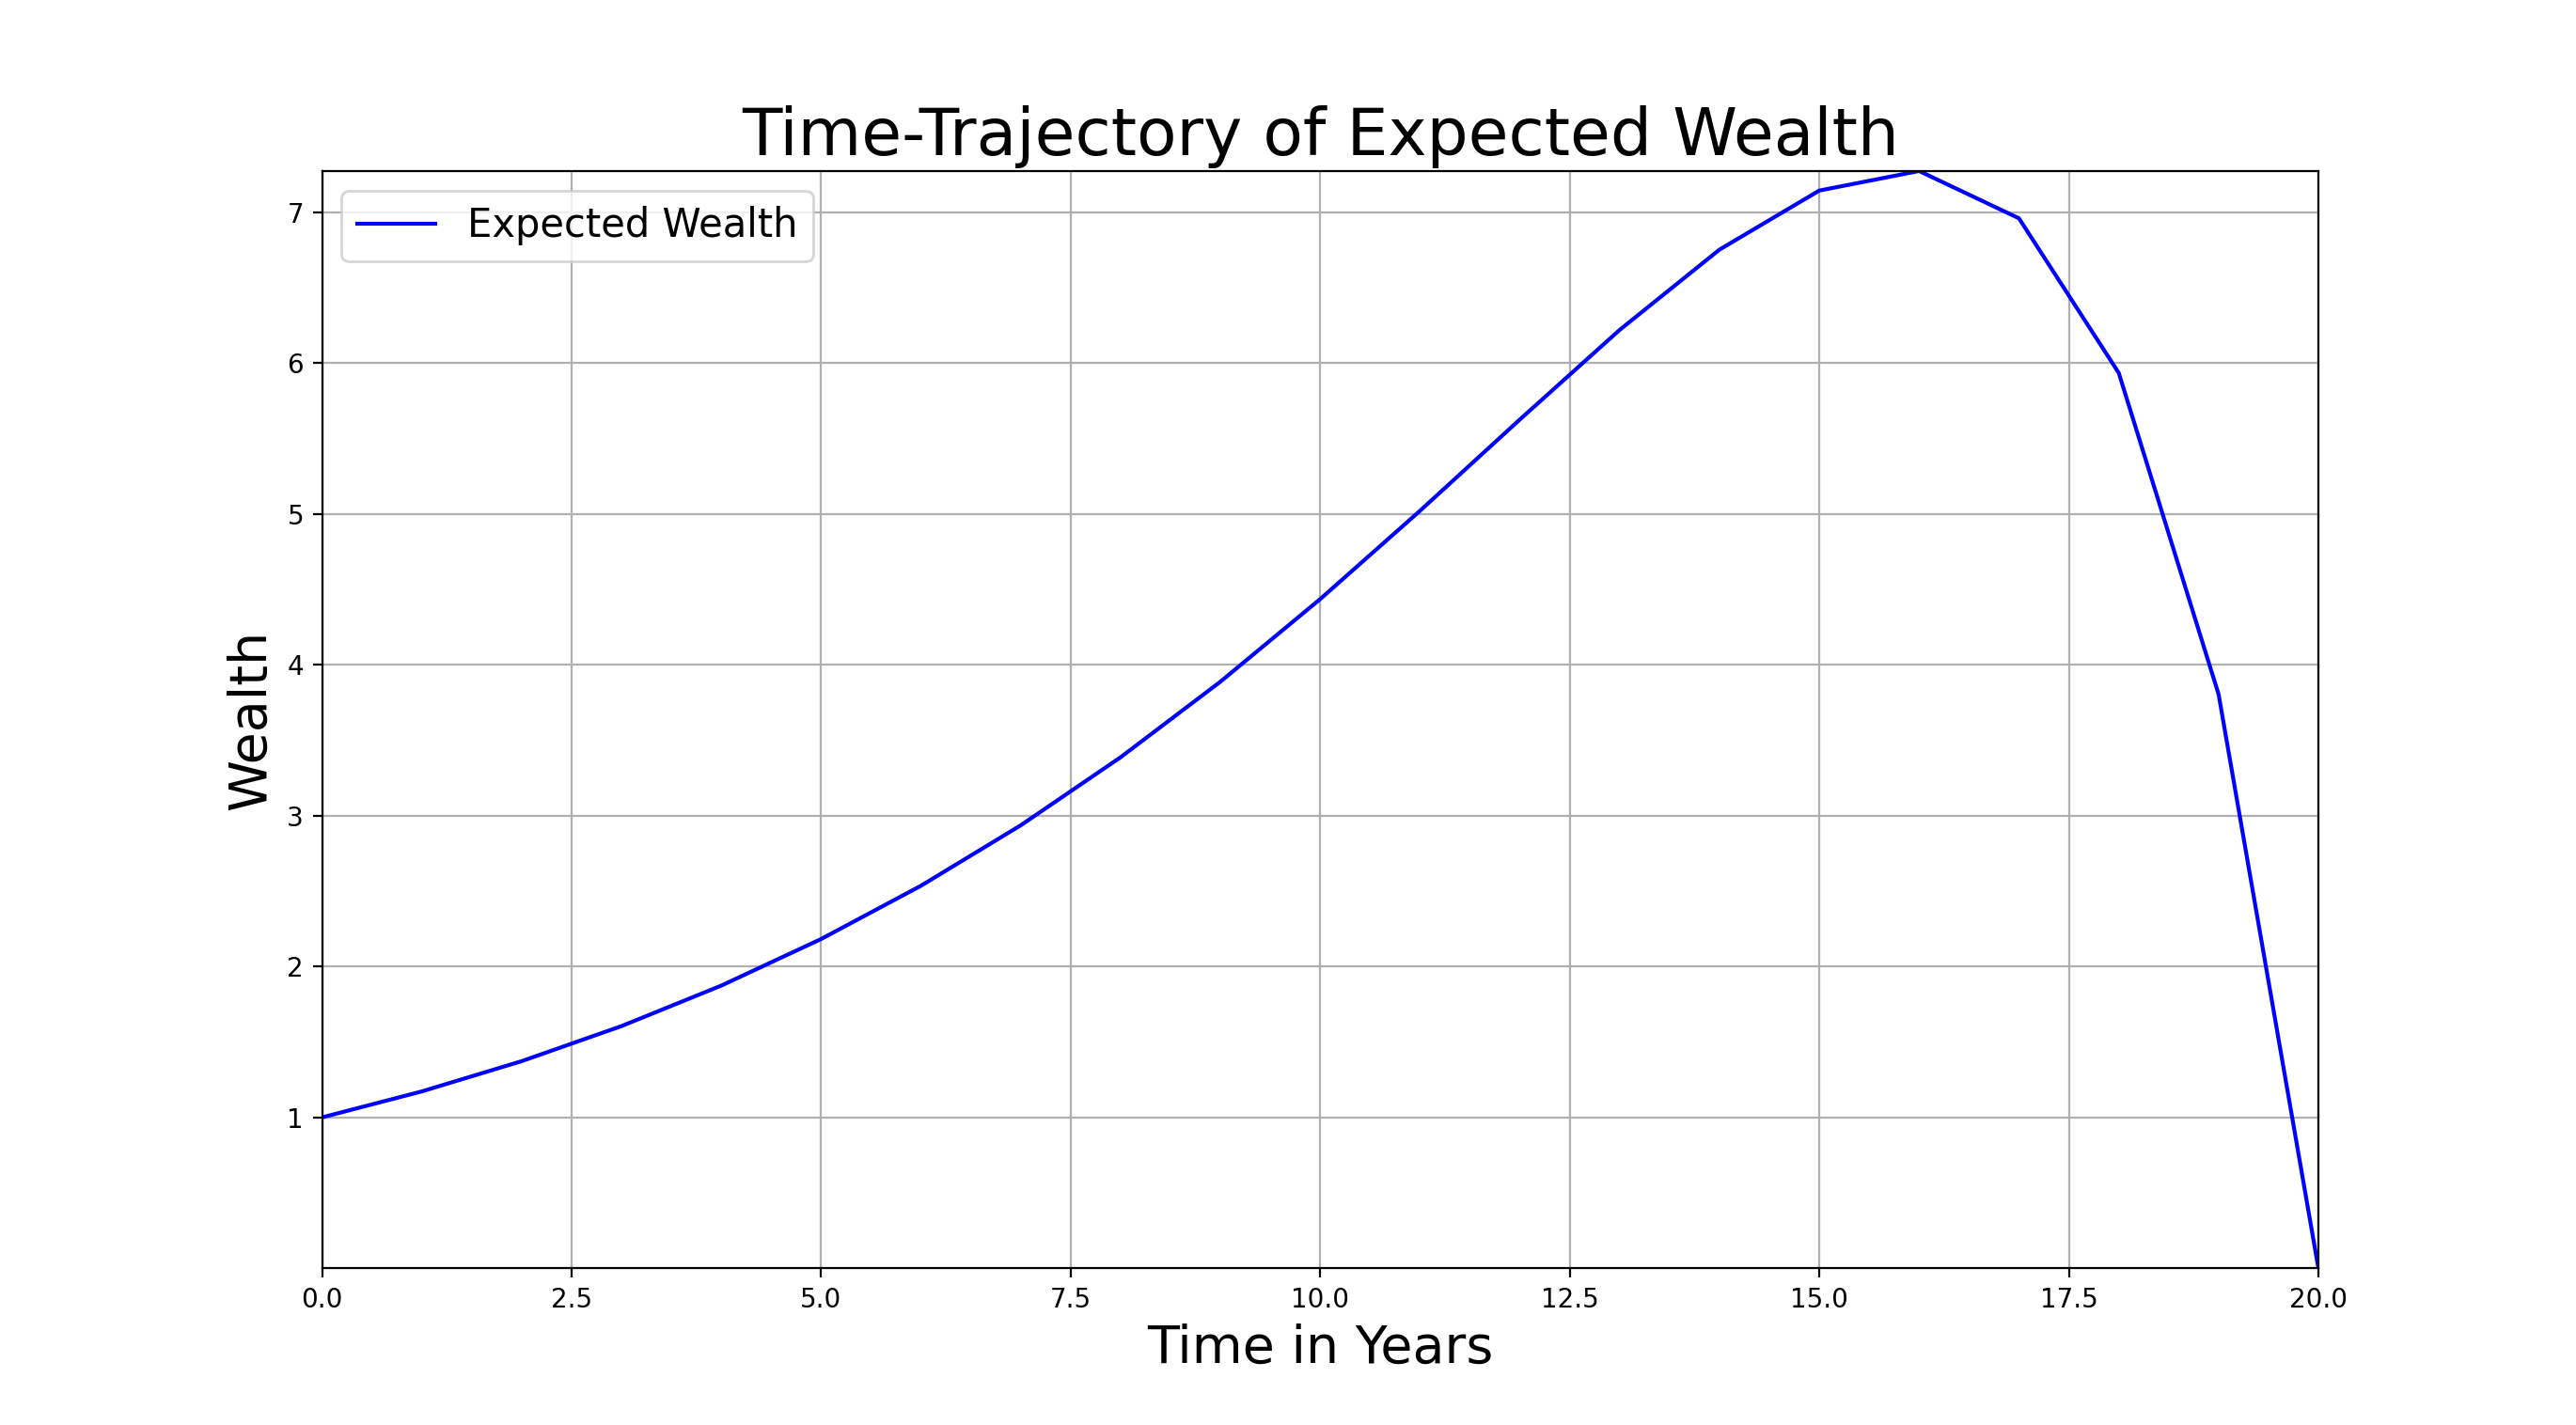
\includegraphics[width=12cm, height=8cm]{wealth_trajectory.png}
\end{frame}

\begin{frame}
\frametitle{Discrete-Time Asset-Allocation Example}
\pause
\begin{itemize}[<+->]
\item At time steps $t = 0, 1, \ldots, T-1$, we can asset-allocate wealth $W_t$
\item 1 risky asset, unconstrained allocation, no transaction costs
\item Risky asset return for each time step $\sim \mathcal{N}(\mu, \sigma^2)$
\item Riskless asset has constant return $r$ for each time step
\item Assume no wealth consumption for any time $t < T$
\item We liquidate and consume wealth $W_T$ at time $T$
\item Goal:  Maximize Expected Utility of Wealth $W_T$ at time $T$
\item Dynamic allocation $x_t \in \mathbb{R}$ in risky asset, $W_t - x_t$ in riskless asset
\item Utility of Wealth $W_T$ at time $T$ is given by CARA function:
$$U(W_T) = \frac {1 - e^{-a W_T}} {a} \text{ for some fixed } a \neq 0$$
\item So we maximize, for each $t=0, 1, \ldots, T-1$, over choices of $x_t \in \mathbb{R}$:
$$\mathbb{E}[\frac {- e^{-a W_T}} a | (t, W_t)]$$
\end{itemize}
\end{frame}

\begin{frame}
\frametitle{MDP for Discrete-Time Asset-Allocation}
\pause
\begin{itemize}[<+->]
\item Continuous-States/Actions, Discrete-Time, Finite-Horizon MDP
\item All states at time $T$ are terminal states
\item {\em State} $s_t \in \mathcal{S}_t$ is the wealth $W_t$, {\em Action} $a_t \in \mathcal{A}_t$ is risky investment $x_t$
\item  Deterministic policy at time $t$ denoted as $\pi_t$, so $\pi_t(W_t) = x_t$
\item Optimal deterministic policy at time $t$ denoted as $\pi^*_t$, so $\pi^*_t(W_t) = x^*_t$
\item Single-time-step return of risky asset from $t$ to $t+1$ is $Y_t \sim \mathcal{N}(\mu, \sigma^2)$
$$W_{t+1} = x_t \cdot (1 + Y_t) + (W_t - x_t) \cdot (1 + r) = x_t \cdot (Y_t - r) + W_t \cdot (1 + r)$$
\item MDP {\em Reward} is 0 for all $t = 0, 1, \ldots, T-1$
\item MDP {\em Reward} at time $T$: $\frac {- e^{-a W_T}} {a}$
\item MDP discount factor $\gamma = 1$
\end{itemize}
\end{frame}

\begin{frame}
\frametitle{Optimal Value Function and Bellman Optimality Equation}
\pause
\begin{itemize}[<+->]
\item Denote Value Function at time $t$ for policy $\pi = (\pi_0, \pi_1, \ldots, \pi_{T-1})$ as:
$$V^{\pi}_t(W_t) = \mathbb{E}_{\pi}[\frac {- e^{-a W_T}} a | (t, W_t)]$$
\item Denote Optimal Value Function at time $t$ as:
$$V^*_t(W_t) = \max_{\pi} V^{\pi}_t(W_t) = \max_{\pi} \{ \mathbb{E}_{\pi}[\frac {- e^{-a W_T}} a | (t, W_t)] \}$$
\item Bellman Optimality Equation is:
$$V^*_t(W_t) = \max_{x_t} \{\mathbb{E}_{Y_t \sim \mathcal{N}(\mu, \sigma^2)}[V^*_{t+1}(W_{t+1})]\}$$
$$V^*_{T-1}(W_{T-1}) = \max_{x_{T-1}} \{ \mathbb{E}_{Y_{T-1} \sim \mathcal{N}(\mu, \sigma^2)}[\frac {- e^{-a W_T}} a] \}$$
\item Make an educated guess for the functional form of the $V^*_t(W_t)$:
$$V^*_t(W_t) = - b_t \cdot e^{-c_t \cdot W_t}$$
where $b_t, c_t$ are independent of the wealth $W_t$
\end{itemize}
\end{frame}


\begin{frame}
\frametitle{Solving the Optimal Value Function}
\pause
\begin{itemize}[<+->]
\item We express Bellman Optimality Equation using this functional form:
\begin{equation*}
\begin{split}
V^*_t(W_t) & = \max_{x_t} \{ \mathbb{E}_{Y_t \sim \mathcal{N}(\mu, \sigma^2)} [-b_{t+1} \cdot e^{-c_{t+1} \cdot W_{t+1}}] \} \\
& = \max_{x_t} \{ \mathbb{E}_{Y_t \sim \mathcal{N}(\mu, \sigma^2)} [-b_{t+1} \cdot e^{-c_{t+1} \cdot (x_t \cdot (Y_t - r) + W_t \cdot (1+r))}] \} \\
& = \max_{x_t} \{-b_{t+1} \cdot e^{-c_{t+1} \cdot (1 + r) \cdot W_t - c_{t+1} \cdot (\mu - r) \cdot x_t + c^2_{t+1} \cdot \frac {\sigma^2} {2} \cdot x_t^2} \}
\end{split}
\end{equation*}
\item The partial derivative of term inside the $\max$ with respect to $x_t$ is 0:
$$ -c_{t+1} \cdot (\mu - r) + \sigma^2 \cdot c^2_{t+1} \cdot x^*_t = 0$$
\begin{equation}
\Rightarrow x^*_t = \frac {\mu - r} {\sigma^2 \cdot c_{t+1}}
\label{eq:pi-star-functional-discrete}
\end{equation}
\end{itemize}
\end{frame}

\begin{frame}
\frametitle{Solving the Optimal Value Function}
\pause
\begin{itemize}[<+->]
\item Next we substitute maximizing $x_t^*$ in Bellman Optimality Equation:
$$V^*_t(W_t) = - b_{t+1} \cdot e^{-c_{t+1} \cdot (1 + r) \cdot W_t - \frac {(\mu - r)^2} {2 \sigma^2}} $$
\item But since $V^*_t(W_t) = -b_t \cdot e^{-c_t \cdot W_t}$, we can write:
$$b_t = b_{t+1} \cdot e^{- \frac {(\mu -r)^2} {2 \sigma^2}}, c_t = c_{t+1} \cdot (1 + r)$$
\item We can calculate $b_{T-1}$ and $c_{T-1}$ from {\em Reward} $\frac {- e^{-a W_T}} a$
$$V^*_{T-1}(W_{T-1}) = \max_{x_{T-1}} \{ \mathbb{E}_{Y_{T-1} \sim \mathcal{N}(\mu, \sigma^2)}[\frac {- e^{-a W_T}} a] \}$$
\item Substituting for $W_T$, we get:
$$V^*_{T-1}(W_{T-1}) = \max_{x_{T-1}} \{ \mathbb{E}_{Y_{T-1} \sim \mathcal{N}(\mu, \sigma^2)}[\frac {- e^{-a (x_{T-1}\cdot (Y_{T-1} - r) + W_{T-1} \cdot (1 + r))}} a] \}$$
\end{itemize}
\end{frame}

\begin{frame}
\frametitle{Solving the Optimal Value Function}
\pause
\begin{itemize}[<+->]
\item The expectation of this exponential (under normal distribution) is:
$$V^*_{T-1}(W_{T-1}) = \frac {-e^{-\frac {(\mu - r)^2} {2 \sigma^2} - a \cdot (1 + r) \cdot W_{T-1}}} a$$
\item This gives us $b_{T-1}$ and $c_{T-1}$ as follows:
$$b_{T-1} = \frac {e^{- \frac {(\mu - r)^2} {2 \sigma^2}}} a$$
$$c_{T-1} = a \cdot (1 + r)$$
\item Now we can unroll recursions for $b_t$ and $c_t$:
$$b_t = \frac {e^{- \frac {(\mu - r)^2 \cdot (T-t)} {2 \sigma^2}}} a$$
$$ c_t = a \cdot (1+ r)^{T-t}$$
\end{itemize}
\end{frame}

\begin{frame}
\frametitle{Solving the Optimal Value Function}
\pause
\begin{itemize}[<+->]
\item Substituting the solution for $c_{t+1}$ in \eqref{eq:pi-star-functional-discrete} gives the Optimal Policy:
$$\pi^*_t(W_t) = x^*_t = \frac {\mu - r} {\sigma^2 \cdot a \cdot (1+ r)^{T-t-1}}$$
\item Note optimal action at time $t$ does not depend on state $W_t$
\item Hence, optimal policy $\pi^*_t(\cdot)$ is a constant deterministic policy function
\item Substituting for $b_t$ and $c_t$  gives us the Optimal Value Function:
$$V^*_t(W_t) = \frac {- e^{- \frac {(\mu - r)^2 (T-t)} {2 \sigma^2}}} a \cdot e^{- a (1+ r)^{T-t} \cdot W_t}$$
\end{itemize}
\end{frame}


\begin{frame}
\frametitle{Real-World}
\pause
\begin{itemize}[<+->]
\item Analytical tractability in Merton's formulation was due to:
\begin{itemize}
\item Normal distribution of asset returns
\item Constant Relative Risk-Aversion
\item Frictionless, continuous trading
\end{itemize}
\item However, real-world situation involves:
\begin{itemize}
\item Discrete amounts of assets to hold and discrete quantities of trades
\item Transaction costs
\item Locked-out days for trading
\item Time-Heterogeneous/arbitrary/correlated processes of multiple assets
\item Changing/uncertain risk-free rate
\item Consumption constraints
\item Arbitrary Risk-Aversion/Utility specification
\end{itemize}
\item $\Rightarrow$ Approximate Dynamic Programming or Reinforcement Learning
\item Large Action Space points to Policy Gradient Algorithms
\end{itemize}
\end{frame}


\begin{frame}[fragile]
\frametitle{Code for Discrete-time Dynamic Asset-Allocation}
\pause
\begin{lstlisting}
@dataclass(frozen=True)
class AssetAllocDiscrete:
    risky_return_distributions: \
        Sequence[Distribution[float]]
    riskless_returns: Sequence[float]
    utility_func: Callable[[float], float]
    risky_alloc_choices: Sequence[float]
    feature_functions: \
        Sequence[Callable[[Tuple[float, float]], float]]
    dnn_spec: DNNSpec
    initial_wealth_distribution: Distribution[float]
\end{lstlisting}    
\end{frame}    

\end{document}